\section{Policy Gradient Methods}

The goal of this problem is to experiment with policy gradient and its variants, including variance reduction methods. Your goal will be to set up policy gradient for both continuous and discrete environments, and implement a neural network baseline for variance reduction. The script for running the policy gradient algorithm is setup in \texttt{run.py}, and everything that you need to implement is in the files \texttt{baseline\_network.py}, \texttt{mlp.py}, \texttt{policy.py} and \texttt{policy\_gradient.py} within the submission folder. Each submission script has detailed instructions for each implementation task. We have also provided an overview of key steps in the algorithm below: \\


\textbf{REINFORCE}

Recall the policy gradient theorem:
\[ \nabla_\theta J(\theta) = \mathbb E_{\pi_\theta} \left[ \nabla_\theta \log\pi_\theta(a \mid s) Q^{\pi_\theta} (s,a) \right] \]
REINFORCE is a Monte Carlo policy gradient algorithm, so we will be using the sampled returns $G_t$ as unbiased estimates of $Q^{\pi_\theta}(s,a)$. 
The REINFORCE estimator can be expressed as the gradient of the following objective function:
\[ J(\theta) = \frac{1}{\sum T_i} \sum_{i=1}^{\mid D \mid} \sum_{t=1}^{T_i} \log(\pi_\theta(a^i_t \mid s^i_t)) G^i_t \]
where $D$ is the set of all trajectories collected by policy $\pi_\theta$, and $\tau^i =(s^i_0, a^i_0, r^i_0, s^i_1, \dots, s^i_{T_i}, a^i_{T_i}, r^i_{T_i})$ is trajectory $i$. \\

\textbf{Baseline}

One difficulty of training with the REINFORCE algorithm is that the Monte Carlo sampled return(s) $G_t$ can have high variance. To reduce variance, we subtract a baseline $b_{\phi}(s)$ from the estimated returns when computing the policy gradient. A good baseline is the state value function, $V^{\pi_\theta}(s)$, which requires a training update to $\phi$ to minimize the following mean-squared error loss:
\[ L_{\text{MSE}}(\phi) = \frac{1}{\sum T_i} \sum_{i=1}^{\mid D \mid} \sum_{t=1}^{T_i} (G^i_t - b_{\phi}(s^i_t))^2\] \\

\textbf{Advantage Normalization}

After subtracting the baseline, we get the following new objective function:

\[ J(\theta) = \frac{1}{\sum T_i} \sum_{i=1}^{\mid D \mid} \sum_{t=1}^{T_i} \log(\pi_\theta(a^i_t \mid s^i_t)) \hat{A}^i_t \]

where

\[\hat{A}^i_t = G^i_t - b_{\phi}(s^i_t)\]

A second variance reduction technique is to normalize the computed advantages, $\hat{A}^i_t$, so that they have mean $0$ and standard deviation $1$. From a theoretical perspective, we can consider centering the advantages to be simply adjusting the advantages by a constant baseline, which does not change the policy gradient. Likewise, rescaling the advantages effectively changes the learning rate by a factor of $1/\sigma$, where $\sigma$ is the standard deviation of the empirical advantages. \\

\textit{Note: for the following coding questions some scripts contain member functions of different classes with the same name. In order to distinguish which function we refer to in each question we use the following syntax ~class::function~.}
\clearpage


\begin{enumerate}[(a)]

	\item \points{1a}

Implement ~build_mlp~ within ~submission/mlp.py~ which will be used to construct a multi layer perceptron based on input argument values.

% Note: The "batch size" for all the arguments is $\sum T_i$ since we already flattened out all the episode observations, actions, and rewards for you.


% We have provided some basic tests to sanity check your implementation. \textbf{Please note that the tests are not comprehensive, and passing them does not guarantee a correct implementation}. Use the following command to run the tests:
% \begin{verbatim}
% python run_basic_tests.py
% \end{verbatim}
% You can also add additional tests of your own design in \texttt{tests/test\_basic.py}.

	\item \points{1b}

Implement the following functions within ~submission/baseline_network.py~ to create the baseline network for our policy gradient implementation: 

\begin{itemize}
	\item ~BaselineNetwork::__init__~ 
	\item ~BaselineNetwork::forward~ 
	\item ~BaselineNetwork::calculate_advantage~ 
	\item ~BaselineNetwork::update_baseline~
\end{itemize}

	\item \points{1c}

Implement ~PolicyGradient::init_policy~ within ~policy_gradient.py~ in order to initialize a network and optimizer for our implementation of policy gradient.

	\item \points{1d}

Implement ~PolicyGradient::get_returns~ within ~policy_gradient.py~ in order to calculate returns $G_{t}$ given data about specific trajectories.

	\item \points{1e}

In this question, we will define the conditional probability distribution over actions for both discrete and continuous environments. Implement the following functions in ~submission/policy.py~ in order to define these distributions and how we sample from them: 

\begin{itemize}
	\item ~BasePolicy::act~ 
	\item ~CategoricalPolicy::action_distribution~ 
	\item ~GaussianPolicy::__init__~ 
	\item ~GaussianPolicy::std~
	\item ~GaussianPolicy::action_distribution~ 
\end{itemize}

	\item \points{1f}

Implement the following functions in ~submission/policy_gradient.py~: 

\begin{itemize}
	\item ~PolicyGradient::update_policy~ 
	\item ~PolicyGradient::normalize_advantage~ 
\end{itemize}

This will complete the ~PolicyGradient~ class by providing a network update rule as well as the option to normalize advantages we have calculated.

	\item \points{2g}

In this question, our grader will evaluate the performance of your linear implementation on the test environment based on the code you have already developed in previous questions in this section (No additional code needs to be written for this question).

If you would like, you can observe the performance metrics of your model through running the following command:

\begin{lstlisting}
$ python run.py --config_filename=q2_linear
\end{lstlisting}

This should train your linear model on the test environment with the configuration defined in ~config/q2_linear.yml~. You may view the evaluation scores from your training run under the following directory ~results/q2_linear/~. We expect your implementation to achieve the optimal return on the test environment. Below we have provided a plot of scores which we expect the scores generated by your implementation to closely resemble:

\begin{figure}[H]
\centering
  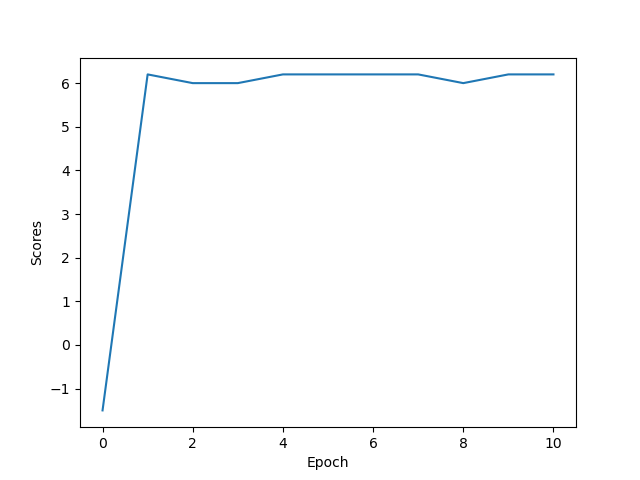
\includegraphics[width=.5\linewidth]{images/linear_test.png}
\end{figure}

\textit{Note: You will be need these results to provide responses to future questions which are made available online via Gradescope.}
\clearpage

\end{enumerate}